\documentclass[tikz]{standalone}
\usepackage{amsmath}

\usetikzlibrary{arrows.meta}
\usetikzlibrary{fadings}
\usetikzlibrary{decorations.markings}

\definecolor{lightblue}{HTML}{2A6EB1}
\definecolor{lightred}{HTML}{FF8181}
\definecolor{darkblue}{rgb}{0.000, 0.275, 0.545}
\definecolor{darkred}{rgb}{0.647,0.129,0.149}
\definecolor{green}{rgb}{0.365, 0.592, 0.157}

\tikzfading[name=fade up, bottom color=transparent!0, top color=transparent!100]

\begin{document}

\begin{tikzpicture}


\node[anchor=north west,inner sep=0] (image) at (0,4.9) {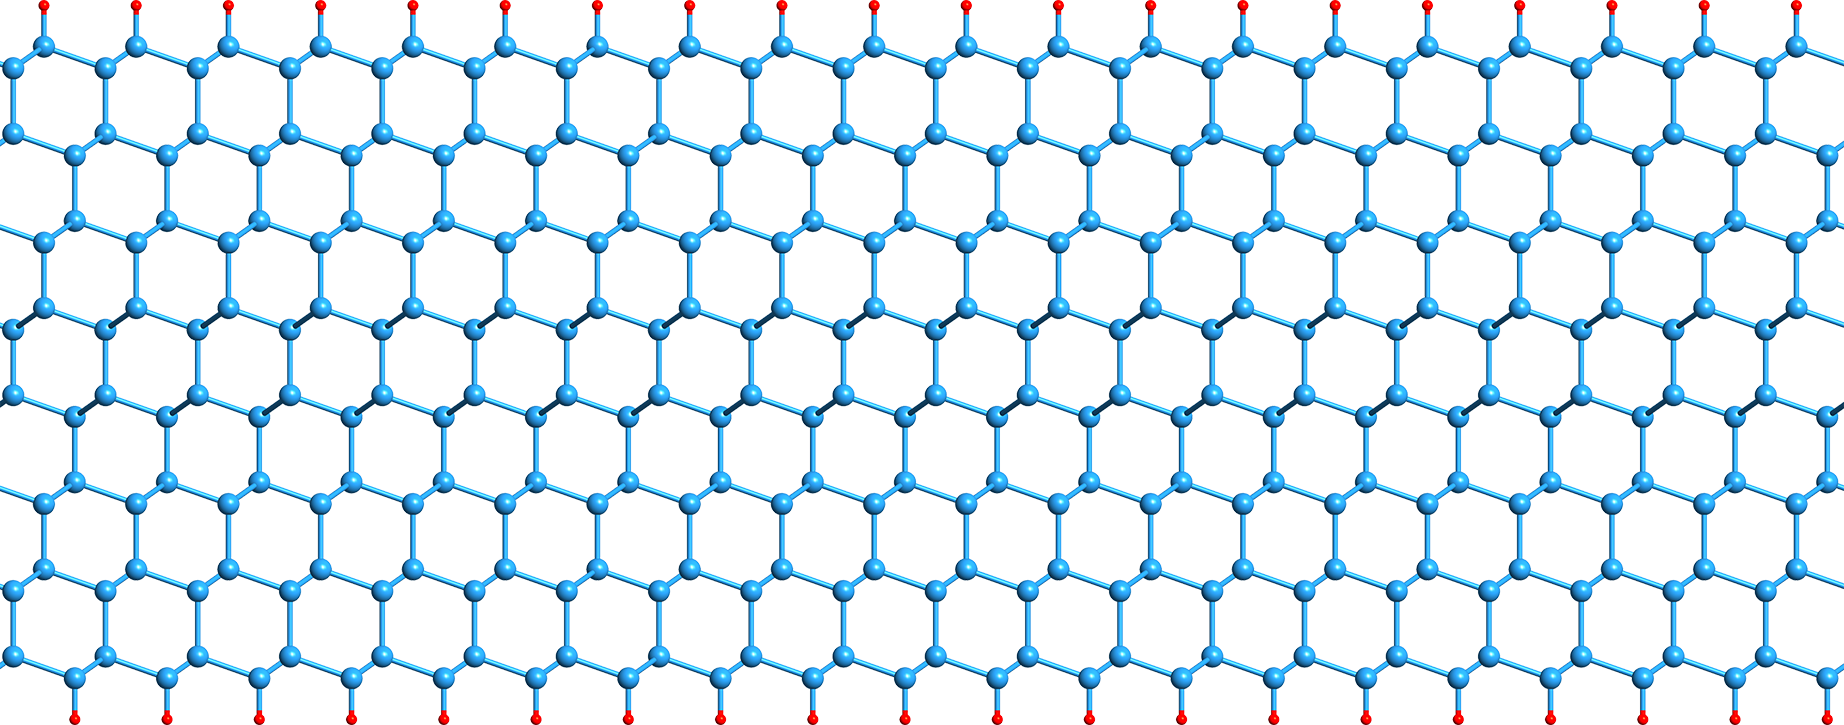
\includegraphics[scale=0.3]{structure/si111-fig.png}};

%%%% colored regions %%%%
\fill [green,fill opacity=0.65] (0,2) rectangle (18,5);
\fill [lightred, fill opacity=0.65] (0,-2) rectangle (18,2);
\fill [white] (18,-2) rectangle (20,5);
\fill [white] (0,-3) rectangle (20,-1.99);
\fill [white,path fading=fade up] (0,-2) rectangle (20,0);
\fill [white,path fading=fade up] (0,-2) rectangle (20,0);


%%%% above the surface %%%%
% axes guide
\draw [very thick] (2,9) +(90:0.8) arc (90:135:0.8);
\draw [Latex-Latex,thick] (2,11) -- ++(0,-2) -- ++(2,0);
\draw [Latex-,ultra thick] (2,9) -- ++(135:2.3);
\draw [color=black] (2,9) circle (0.10);
\node at (1.6,10.1) {\LARGE $\theta_{0}$};
\node at (0.7,9.8) {\LARGE $\boldsymbol{\nu}_{v}$};
\node at (2.4,11) {\LARGE $z$};
\node at (2,8.6) {\LARGE $\hat{\mathbf{s}}$};
\node at (4.2,8.8) {\LARGE $\hat{\boldsymbol{\kappa}}$};
% arrows
\draw [thick] (8.893,8.75) -- ++(-60:0.41) -- ++(-150:0.41); % right angle
\draw [ultra thick,darkblue,dash pattern=on 25pt off 2pt on 5pt off 2pt on 3pt off 2pt on 1pt off 2pt] (8.893,8.75) -- ++(30:6);
\draw [-Latex,ultra thick,darkblue] (2.4,5) -- ++(30:12.2);
\draw [-Latex,ultra thick,darkblue] (2.4,5) -- ++(30:7.1);
\draw [-Latex,ultra thick,darkblue] (2.4,5) -- ++(30:1.8);


%%%% inside slab %%%%
% first beam from the left
\draw [darkred,line width=2pt,dashed] (0,2.9) -- (18,2.9);
\draw [-Latex,ultra thick,lightblue] (0.3,2.9) -- ++(45:2.97);
\draw [-Latex,ultra thick,lightblue] (0.3,2.9) -- ++(-37:1.49);
\draw [ultra thick,lightblue,dash pattern=on 39pt off 2pt on 5pt off 2pt on 3pt off 2pt on 1pt off 2pt] (1.5,2) -- ++(-75:2);
\filldraw [darkred] (0.3,2.9) circle (0.15);

% first node on upper surface at (4.5,5)
\draw [thick,dashed] (4.5,5) -- ++(120:1);
\draw [ultra thick,lightblue,dash pattern=on 25pt off 2pt on 5pt off 2pt on 3pt off 2pt on 1pt off 2pt] (4.5,5) -- ++(30:1.5);
\draw [Latex-,ultra thick,lightblue] (4.5,5) -- ++(-135:4.25);
\draw [-Latex,ultra thick,lightblue] (4.5,5) -- ++(-45:4.25);
\draw [ultra thick,lightblue,dash pattern=on 39pt off 2pt on 5pt off 2pt on 3pt off 2pt on 1pt off 2pt] (7.5,2) -- ++(-75:2);
% second node on upper surface at (10.6,5)
\draw [thick,dashed] (10.6,5) -- ++(120:4.1);
\draw [ultra thick,lightblue,dash pattern=on 25pt off 2pt on 5pt off 2pt on 3pt off 2pt on 1pt off 2pt] (10.5,5) -- ++(30:1.5);
\draw [Latex-,ultra thick,lightblue] (10.5,5) -- ++(-135:4.25);
\draw [-Latex,ultra thick,lightblue] (10.5,5) -- ++(-45:4.25);
\draw [ultra thick,lightblue,dash pattern=on 39pt off 2pt on 5pt off 2pt on 3pt off 2pt on 1pt off 2pt] (13.5,2) -- ++(-75:2);
% third node on upper surface at (16.5,5)
\draw [thick,dashed] (16.5,5) -- ++(120:7.1);
\draw [ultra thick,lightblue,dash pattern=on 25pt off 2pt on 5pt off 2pt on 3pt off 2pt on 1pt off 2pt] (16.5,5) -- ++(30:1.5);
\draw [Latex-,ultra thick,lightblue] (16.5,5) -- ++(-135:4.25);
\draw [ultra thick,lightblue,dash pattern=on 25pt off 2pt on 5pt off 2pt on 3pt off 2pt on 1pt off 2pt] (16.5,5) -- ++(-45:1.5);


%%%% labels %%%%
\node [anchor=east] at (0.1,2.9) {\LARGE $\boldsymbol{\mathcal{P}}(2\omega)$};
% z_n and distace arrows
\node [scale = 2] at (-0.4,4.1) {$z_{n}$};
\draw [Latex-Latex,ultra thick] (0.3,3.06) -- (0.3,5);
% side labels
\node [anchor=west, scale = 2, align=center] at (18,6.5) {Vacuum\\($\epsilon_{v}=1$)};
\node [anchor=west, scale = 2, align=left] at (18,3.5) {Surface\\Layer ($\epsilon_{\ell}$)};
\node [anchor=west, scale = 2, align=center] at (18,0.5) {Bulk ($\epsilon_{b}$)};
\node [anchor=east, scale = 2, align=left] at (0,5.1) {$z = 0$};
\node [anchor=east, scale = 2, align=left] at (0,2.1) {$z = -d$};
% surface lines
\draw [ultra thick] (0,5) -- (18,5);
\draw [ultra thick] (0,2) -- (18,2);

% \node [scale = 2] at (17.5,3.5) {$\epsilon_{\ell}$};
% \node [anchor=east, scale = 2] at (0,6.5) {$\epsilon_{v}=1$};
% \node [scale = 2] at (17.5,1) {$\epsilon_{b}$};


\end{tikzpicture}

\end{document}
